% Provenance (never printed): see sources/outline_sources.md (Year 2: fractional
% crystallisation, Bowen's series, compatible and incompatible elements, mixing and
% assimilation, layered intrusions).
% Curves from figdata/bachelor-2/differentiation.py (Bowen 1913 plagioclase loop, Rayleigh and
% equilibrium laws, Wilcox 1954 Paricutin analyses and mass balance, AFC closed form,
% Tegner et al. 2023 Skaergaard whole-rock data); exercise and problem values in the Book 4
% scratch calculator calc/ch08.py.
\chapter{岩浆分异}\label{ch:b2:magmatic-differentiation}

1943 年 2 月 20 日，墨西哥西部一座火山开始喷发，
持续了九年。其早期熔岩为玄武质安山岩，二氧化硅含量 \qty{55}{\percent}；
末期熔岩（1952 年 2 月）为安山岩，二氧化硅含量略高于
\qty{60}{\percent}。帕里库廷火山在此期间没有迁移到另一个
喷口，其熔岩随喷出先后被逐一分析。其下方的\omterm{def:b2:magma-emplacement:magma}{岩浆}
自身发生了变化：它长出晶体并将其留在身后，还吞食了
周围的一些花岗质岩石。以玄武岩形式离开地幔的\omterm{def:b2:magma-emplacement:magma}{岩浆}可以
最终成为流纹岩，沿途留下的岩石记录了它的变化过程。
本章跟踪一个冷却中的\omterm{def:b2:magma-emplacement:magma}{岩浆}：矿物的结晶顺序、
描述晶体移出时主量元素与\omterm{def:b2:elements-in-the-earth:trace}{微量元素}变化的规律、
由这些晶体组成的岩石，以及\omterm{def:b2:magma-emplacement:magma}{岩浆}吸纳
另一\omterm{def:b2:magma-emplacement:magma}{岩浆}或地壳时发生的情况。
% ledger: wilcox54:paricutin

\begin{recall}
\textbf{来自高中分册}：火成岩及其结构；玄武质\omterm{def:b2:magma-emplacement:magma}{岩浆}
中矿物的结晶顺序，橄榄石最先、石英最后；
由鲍文的实验得出。\textbf{来自化学系列本科二年级分册}：
二元相图、固溶体与杠杆规则。\textbf{来自本科一年级分册}：
斜长石，为钙长石 \ce{CaAl2Si2O8} 与钠长石
\ce{NaAlSi3O8} 之间的固溶体，以及其他造岩硅酸盐；薄片
在正交偏光下观察。\textbf{来自\cref{ch:b2:elements-in-the-earth}}：矿物–熔体及总
分配系数 $\bar D = \sum_i x_i D_i$，相容与\omterm{def:b2:elements-in-the-earth:partition}{不相容
元素}、\omterm{def:b2:elements-in-the-earth:normalised}{标准化图解}及\omterm{prop:b2:elements-in-the-earth:normalised}{铕异常}。\textbf{来自
\cref{ch:b2:isotope-geochemistry}}：同位素比值作示踪剂，以及\omterm{prop:b2:isotope-geochemistry:mixing}{混合
双曲线}。\textbf{来自\cref{ch:b2:mantle-melting}}：透辉石–钙长石
低共熔点、\omterm{def:b2:mantle-melting:peritectic}{不一致熔融}、\omterm{def:b2:mantle-melting:ternary}{三元相图}和\omterm{def:b2:mantle-melting:primary}{原生岩浆}。
\end{recall}

\section{结晶顺序}\label{sec:b2:magmatic-differentiation:sequences}

玄武质\omterm{def:b2:magma-emplacement:magma}{岩浆}并非同时结晶出全部矿物。鲍文通过
实验发现，橄榄石通常最先结晶，温度为 1200 至
\qty{1300}{\celsius}；富钙斜长石开始结晶的温度
与辉石大致相当；最后富含二氧化硅的液体结晶出钾长石、石英和
或许还有白云母，温度约 750 至 \qty{800}{\celsius}。两者之间，
镁铁质矿物并非简单堆积：每种矿物都与液体反应，生成下一种矿物。
% ledger: earle:bowen (Book 2), tulane:bowen (Book 2)

\begin{definition}[鲍文反应系列]\label{def:b2:magmatic-differentiation:bowen}
\emph{鲍文反应系列}\index{鲍文反应系列}是常见硅酸盐从冷却的玄武质\omterm{def:b2:magma-emplacement:magma}{岩浆}中结晶的顺序，
分为两支，
两支在末端相交。在\emph{不连续支}中，每种镁铁质矿物
与液体反应，生成另一种结构的新矿物：橄榄石、
辉石、角闪石、黑云母。在\emph{连续支}中，斜长石持续结晶，
其成分由富钙连续变化为
富钠。最后的液体结晶出钾长石、白云母和
石英。
\end{definition}
% ledger: earle:bowen (Book 2)

\begin{omfigure}
\centering
\begin{tikzpicture}[font=\small, x=1cm, y=1cm,
  mn/.style={draw, rounded corners=2pt, fill=white, inner sep=3pt, minimum width=2.3cm,
             align=center}]
\draw[-{Stealth[length=4pt]}, thick, gray] (-1.3,0.3) -- (-1.3,-6.0);
\node[rotate=90, anchor=south, font=\scriptsize, gray] at (-1.4,-2.85) {温度下降};
\node[anchor=east, font=\scriptsize] at (-1.5,0) {$\approx$ 1200--\qty{1300}{\celsius}};
\node[anchor=east, font=\scriptsize] at (-1.5,-5.6) {$\approx$ 750--\qty{800}{\celsius}};
\node[mn] (ol) at (1,0) {橄榄石};
\node[mn] (px) at (1,-1.4) {辉石};
\node[mn] (am) at (1,-2.8) {角闪石};
\node[mn] (bt) at (1,-4.2) {黑云母};
\draw[-{Stealth[length=4pt]}, thick] (ol) -- (px);
\draw[-{Stealth[length=4pt]}, thick] (px) -- (am);
\draw[-{Stealth[length=4pt]}, thick] (am) -- (bt);
\node[font=\scriptsize, align=center] at (1,0.8) {不连续支 \\（每一步形成一种新矿物）};
\node[mn] (ca) at (6,-1.4) {富钙 \\斜长石};
\node[mn] (na) at (6,-4.2) {富钠 \\斜长石};
\fill[left color=white, right color=white, top color=orange!35, bottom color=orange!8]
  (5.75,-2.0) rectangle (6.25,-3.6);
\draw[-{Stealth[length=4pt]}, thick] (ca) -- (na);
\node[font=\scriptsize, align=center] at (6,0.8) {连续支 \\（一种矿物，成分连续变化）};
\node[mn, minimum width=7.2cm] (last) at (3.5,-5.6) {钾长石、白云母、石英};
\draw[-{Stealth[length=4pt]}, thick] (bt) -- (bt|-last.north);
\draw[-{Stealth[length=4pt]}, thick] (na) -- (na|-last.north);
\end{tikzpicture}
\par\smallskip{\small \omterm{def:b2:magmatic-differentiation:bowen}{鲍文反应系列}。橄榄石与富钙斜长石
在玄武质\omterm{def:b2:magma-emplacement:magma}{岩浆}中最先结晶；左侧每种镁铁质矿物与液体反应，
生成下一种矿物，右侧斜长石中钠含量不断增高；
最后富含二氧化硅的液体结晶出钾长石、白云母和石英。
图中温度为低压下玄武质\omterm{def:b2:magma-emplacement:magma}{岩浆}的典型值。}
\end{omfigure}
% ledger: earle:bowen (Book 2)

两支分别对应
\cref{ch:b2:mantle-melting}中的两类相图。不连续反应即
顽火辉石的\omterm{def:b2:mantle-melting:peritectic}{不一致熔融}逆向进行：镁橄榄石晶体与富含二氧化硅的液体反应，
生成顽火辉石。连续支是一种固溶体。鲍文于 1913 年
在人工合成的斜长石上进行实验，将每种成分保持在已知温度，并
观察玻璃相与晶体：钙长石在 \qty{1550}{\celsius} 熔化，钠长石约在
\qty{1100}{\celsius} 熔化，中间成分的斜长石则在
下方曲线（固相线）与上方曲线（液相线）之间的区间内熔化
（见下图）。
% ledger: bowen13:plagioclase, bowen14:mgo-sio2

\begin{omfigure}
\centering
\begin{tikzpicture}
\begin{axis}[omrecord, width=0.78\linewidth, height=6.4cm,
  xmin=0, xmax=100, ymin=1050, ymax=1600,
  xlabel={钙长石分子含量（\unit{\percent}）}, ylabel={温度（\unit{\celsius}）},
  y tick label style={/pgf/number format/1000 sep={}}, unbounded coords=discard,
  tick label style={font=\scriptsize}, label style={font=\small}]
\addplot[very thick, black] table[x=an, y=T_liq] {figdata/out/bachelor-2-differentiation-plag-curve.dat};
\addplot[very thick, black, dashed] table[x=an, y=T_sol] {figdata/out/bachelor-2-differentiation-plag-curve.dat};
\addplot[only marks, mark=*, mark size=1.5pt, blue!70!black] table[x=an, y=T_liq] {figdata/out/bachelor-2-differentiation-plag-data.dat};
\addplot[only marks, mark=o, mark size=1.7pt, blue!70!black] table[x=an, y=T_sol] {figdata/out/bachelor-2-differentiation-plag-data.dat};
\draw[densely dotted, red!70!black, thick] (axis cs:50,1560) -- (axis cs:50,1287);
\draw[red!70!black, thick] (axis cs:50,1450) -- (axis cs:80.6,1450);
\draw[red!70!black, thick] (axis cs:33.3,1394) -- (axis cs:70.6,1394);
\draw[red!70!black, thick] (axis cs:13.9,1287) -- (axis cs:50,1287);
\addplot[only marks, mark=*, mark size=1.4pt, red!70!black] coordinates {(50,1450) (80.6,1450) (33.3,1394) (70.6,1394) (13.9,1287) (50,1287)};
\node[font=\scriptsize] at (axis cs:30,1530) {液体};
\node[font=\scriptsize, align=center] at (axis cs:83,1200) {斜长石 \\（固溶体）};
\node[font=\scriptsize, anchor=west] at (axis cs:2,1430) {液相线（实线）};
\node[font=\scriptsize, anchor=west] at (axis cs:42,1160) {固相线（虚线）};
\node[font=\scriptsize, anchor=south, red!70!black, fill=white, inner sep=1pt] at (axis cs:68,1452) {\qty{1450}{\celsius}};
\node[font=\scriptsize, anchor=north, red!70!black, fill=white, inner sep=1pt] at (axis cs:31,1284) {\qty{1287}{\celsius}};
\end{axis}
\end{tikzpicture}
\par\smallskip{\small 常压下的斜长石系列，数据取自鲍文（1913）的
淬火实验：熔化开始（圆圈）与熔化完成（圆点）的
熔化温度，曲线经过测量值绘制。红色为
含钙长石 \qty{50}{\percent} 的液体的\omterm{def:b2:magmatic-differentiation:crystallisation}{平衡结晶}：首个晶体
在 \qty{1450}{\celsius} 时析出，钙长石含量 \qty{81}{\percent}；在 \qty{1394}{\celsius}
时，\qty{71}{\percent} 的晶体与 \qty{33}{\percent} 的液体共存；最后的
液体在 \qty{1287}{\celsius} 时钙长石含量为 \qty{14}{\percent}（见\cref{exo:b2:magmatic-differentiation:1}）。}
\end{omfigure}
% ledger: bowen13:plagioclase

液体结晶出固溶体时，会富集
熔点较低的组分：由钙长石含量为 \qty{50}{\percent} 的液体首先析出的斜长石
钙长石含量为 \qty{81}{\percent}，液体则向钠长石方向移动。
之后会发生什么，取决于
晶体是否仍与液体保持平衡。

\begin{definition}[平衡结晶与分离结晶]
\label{def:b2:magmatic-differentiation:crystallisation}
在\emph{平衡结晶}\index{平衡结晶}中，晶体
始终与全部液体保持化学平衡，直至
结束；晶体随液体成分变化而重新达到平衡，体系最终成分
与起始成分相同。在\emph{分离结晶}\index{分离结晶}中，
每个晶体一旦形成，便脱离与液体的反应，
其方式可以是沉降、附着在\omterm{def:b2:magma-emplacement:magma}{岩浆}房壁上，或
被后续生长所包裹；此后液体的演化
如同晶体已被移出体系一样。
\end{definition}

在\omterm{def:b2:magmatic-differentiation:crystallisation}{平衡结晶}中，上图中的斜长石在生长过程中钙长石含量由
\qty{81}{\percent} 变为 \qty{50}{\percent}，每个晶体都
通过扩散与液体重新达到平衡，最后的液体在
固相线 \qty{1287}{\celsius} 处消失。长石中的扩散很慢，天然
晶体往往跟不上：每个晶体的内部与液体隔绝，
液体则如同\omterm{def:b2:magmatic-differentiation:crystallisation}{分离结晶}那样演化，并可以继续向
接近钠长石的成分演化。本章最后一节的图给出了两种路径的计算结果。
% ledger: bowen13:plagioclase

\begin{definition}[液相演化线]\label{def:b2:magmatic-differentiation:lld}
\omterm{def:b2:magma-emplacement:magma}{岩浆}的\emph{液相演化线}\index{液相演化线}是其液体在结晶过程中
所经历的成分序列，可在变异图或
相图上绘出。
\end{definition}

\omterm{def:b2:magmatic-differentiation:lld}{液相演化线}仅是液体的性质。夹带晶体喷出的熔岩
并不严格位于该线上。威尔科克斯在研究帕里库廷的熔岩时，
同时使用了全岩分析结果，以及
通过扣除晶体计算得到的基质（即液体部分）成分。
% ledger: wilcox54:groundmass

\section{主量元素的分离结晶}\label{sec:b2:magmatic-differentiation:majors}

扣除晶体会以简单的线性方式改变液体的成分，
而最早用于读取这一变化的工具，是以二氧化硅为横坐标绘制各氧化物含量的图。

\begin{definition}[哈克图解]\label{def:b2:magmatic-differentiation:harker}
\emph{哈克图解}\index{哈克图解}（二氧化硅变异图）将一组相关岩石中
每种氧化物的质量百分数，相对于其
\ce{SiO2} 质量百分数作图，每种氧化物一个子图。
\end{definition}


帕里库廷的熔岩呈现出此类趋势（\omterm{def:b2:magmatic-differentiation:harker}{哈克图解}见下一命题之后）。
随着二氧化硅含量升高，氧化镁、氧化钙和氧化铝下降，氧化钾上升。
这正是去除橄榄石和斜长石会造成的结果：
橄榄石带走氧化镁和氧化铁，斜长石带走氧化钙和氧化铝，两者都使
液体中二氧化硅和碱金属氧化物含量相对升高。已知矿物的去除能否
定量地解释这些趋势，是一个质量平衡问题。

\begin{proposition}[晶体移除的质量平衡]\label{prop:b2:magmatic-differentiation:lever}
设母\omterm{def:b2:magma-emplacement:magma}{岩浆}的成分为 $\mathbf p$（氧化物质量分数构成的矢量），
它结晶出成分分别为 $\mathbf m_1, \dots, \mathbf m_k$ 的矿物，其质量
分别为每单位母\omterm{def:b2:magma-emplacement:magma}{岩浆}质量中的 $x_1, \dots, x_k$，并设 $\mathbf d$ 为
剩余液体的成分。则
\[
\mathbf p = \Big(1 - \sum_i x_i\Big)\mathbf d + \sum_i x_i \mathbf m_i .
\]
对于单一矿物，母\omterm{def:b2:magma-emplacement:magma}{岩浆}位于连接液体与该矿物的
线段上，在每一张变异图上均如此，被移除的质量分数为
$x = (p_j - d_j)/(m_j - d_j)$（对任一氧化物 $j$ 均成立）：即杠杆规则。
\end{proposition}

\begin{proof}
每种氧化物都守恒：单位质量母\omterm{def:b2:magma-emplacement:magma}{岩浆}中质量为 $p_j$ 的氧化物 $j$，
要么进入液体（液体质量为 $1 - \sum_i x_i$，浓度为 $d_j$），
要么进入矿物。对每个 $j$ 写出上式即得该矢量方程。若只有一种矿物，
方程为 $\mathbf p = (1-x)\mathbf d + x\mathbf m$，
即它是从 $\mathbf d$ 到 $\mathbf m$ 的线段上的一点，
在任一对坐标轴上，该点将线段按 $x : (1-x)$ 分割；解出一个分量即得 $x$。
\end{proof}

\begin{omfigure}
\centering
\begin{tikzpicture}
\begin{groupplot}[group style={group size=2 by 2, horizontal sep=1.6cm, vertical sep=1.3cm},
  width=0.44\linewidth, height=4.3cm, omrecord, xmin=54.5, xmax=60.8,
  tick label style={font=\scriptsize}, label style={font=\small},
  xtick={55,56,57,58,59,60}]
\nextgroupplot[ylabel={\ce{MgO} (\unit{\percent})}, ymin=3.2, ymax=6.0]
\addplot[only marks, mark=*, mark size=1.3pt, blue!70!black] table[x=SiO2, y=MgO] {figdata/out/bachelor-2-differentiation-paricutin.dat};
\nextgroupplot[ylabel={\ce{CaO} (\unit{\percent})}, ymin=6.0, ymax=7.6]
\addplot[only marks, mark=*, mark size=1.3pt, blue!70!black] table[x=SiO2, y=CaO] {figdata/out/bachelor-2-differentiation-paricutin.dat};
\nextgroupplot[ylabel={\ce{K2O} (\unit{\percent})}, ymin=0.7, ymax=1.9, xlabel={\ce{SiO2} (\unit{\percent})}]
\addplot[only marks, mark=*, mark size=1.3pt, blue!70!black] table[x=SiO2, y=K2O] {figdata/out/bachelor-2-differentiation-paricutin.dat};
\node[font=\scriptsize, anchor=west] at (axis cs:55.1,0.80) {1943};
\node[font=\scriptsize, anchor=east] at (axis cs:60.0,1.82) {1952};
\nextgroupplot[ylabel={\ce{Al2O3} (\unit{\percent})}, ymin=17.0, ymax=19.0, xlabel={\ce{SiO2} (\unit{\percent})}]
\addplot[only marks, mark=*, mark size=1.3pt, blue!70!black] table[x=SiO2, y=Al2O3] {figdata/out/bachelor-2-differentiation-paricutin.dat};
\end{groupplot}
\end{tikzpicture}
\par\smallskip{\small 帕里库廷的 22 件熔岩的\omterm{def:b2:magmatic-differentiation:harker}{哈克图解}，
由威尔科克斯（1954）分析，喷发时间自 1943 年 2 月（二氧化硅含量最低）至 1952 年 2 月。
二氧化硅含量每升高 5 个百分点，氧化镁、氧化钙和氧化铝下降，氧化钾
约增加一倍。}
\end{omfigure}
% ledger: wilcox54:table2, wilcox54:paricutin

若有多种矿物，则需联立求解
与氧化物数目相同的守恒方程，才能求得各矿物的质量。威尔科克斯于 1954 年用图解法
完成了这一工作；如今它只是一个小型线性方程组。

\begin{method}[最小二乘质量平衡]\label{met:b2:magmatic-differentiation:massbalance}
为检验子代液体 $\mathbf d$ 是否可由母体 $\mathbf p$ 通过
移除矿物 $\mathbf m_1, \dots, \mathbf m_k$（必要时加入一种
被同化岩石，以负质量计入）而得到，可按如下步骤进行：（1）对每种氧化物 $j$，写出
命题的守恒，整理为关于
每 \qty{100}{g} 母体所移除质量的线性方程，
\[
\sum_i x_i\,(m_{ij} - d_j) = 100\,(p_j - d_j);
\]
（2）取恰好 $k$ 种氧化物，选择受矿物影响变化最大的那些，求解
$k \times k$ 方程组；若氧化物更多，则用最小二乘法求解
（使两边之差的平方和最小）；（3）由求得的质量重新计算子代液体，
并与分析结果逐一氧化物比较：残差
大于分析误差，或某矿物质量为负，则否定该模型。
\end{method}

威尔科克斯选取二氧化硅、氧化铝和氧化镁作为三个对照，并选取三种
材料：组成为 Fo$_{80}$ 的橄榄石、An$_{70}$ 的斜长石，以及
熔岩中所含四个花岗质捕虏体的平均值（\qty{72.5}{\percent} \ce{SiO2}，\qty{3.6}{\percent}
\ce{K2O}）。他指出，仅用橄榄石与斜长石的任何组合
都无法拟合该系列，并表明加入 \qty{25.4}{g} 捕虏体，
并移除 \qty{2.9}{g} 橄榄石和 \qty{9.6}{g} 斜长石，
以 \qty{100}{g} 第一次熔岩的基质为起点，可得 \qty{112.9}{g} 的物质，
与 1950 年熔\omterm{def:b2:magma-emplacement:bodies}{岩基}质相近。精确求解他的三个方程，
得 \qty{24.6}{g}、\qty{3.1}{g} 和 \qty{9.9}{g}；以七种氧化物做最小二乘，
得到不同的结果 \qty{28.7}{g}、\qty{2.4}{g} 和 \qty{5.7}{g}，
可见结果依赖于所选的对照。无论哪种方式，\omterm{def:b2:magma-emplacement:magma}{岩浆}吸收的花岗岩
都多于其结晶量。帕里库廷的熔岩记录了一个开口系统，
即上一节的主题。
% ledger: wilcox54:mass-balance, wilcox54:xenoliths, wilcox54:groundmass

\section{微量元素}\label{sec:b2:magmatic-differentiation:trace}

\omterm{def:b2:elements-in-the-earth:trace}{微量元素}不改变结晶出的矿物，而是随这些矿物，
按其总分配系数 $\bar D$（\cref{ch:b2:elements-in-the-earth}）在各时刻
正在形成的晶体与液相之间分配，此处记为 $D$。

\begin{theorem}[瑞利分馏定律]\label{thm:b2:magmatic-differentiation:rayleigh}
在理想的\omterm{def:b2:magmatic-differentiation:crystallisation}{分离结晶}过程中，若总分配系数
$D$ 为常数，则\omterm{def:b2:elements-in-the-earth:trace}{微量元素}在液相中的浓度满足
\[
\frac{C_L}{C_0} = F^{\,D-1},
\]
其中 $C_0$ 为初始液相中的浓度，$F$ 为剩余
液相的质量分数。这就是\emph{瑞利分馏定律}\index{瑞利分馏定律}
。
\end{theorem}

\begin{proof}
设 $M$ 为液体质量。当析出微小质量 $-\mathrm dM > 0$ 的晶体
形成时仅在该瞬间与液相平衡，其所携带元素的浓度为
$DC_L$。因此液相中元素的质量 $MC_L$ 的变化量为
$\mathrm d(MC_L) = DC_L\,\mathrm dM$。展开得 $M\,\mathrm dC_L = (D-1)C_L\,
\mathrm dM$，故 $\mathrm dC_L/C_L = (D-1)\,\mathrm dM/M$。自 $M_0$ 积分，
此时 $C_L = C_0$，得 $\ln(C_L/C_0) = (D-1)\ln(M/M_0)$，且 $F = M/M_0$。
\end{proof}

\begin{proposition}[微量元素的平衡结晶]
\label{prop:b2:magmatic-differentiation:equilibrium}
若晶体始终与液相保持平衡，则 $C_L/C_0 = 1/(D + F(1-D))$。
\end{proposition}

\begin{proof}
全部晶体的质量 $1-F$（以单位初始质量计）中含有 $DC_L$ 的元素，
因此元素的质量守恒为 $C_0 = FC_L + (1-F)DC_L$。
\end{proof}

\begin{corollary}[不相容元素的比值]\label{cor:b2:magmatic-differentiation:ratio}
对分配系数分别为 $D_1$ 和 $D_2$ 的两种元素，二者在液相中的浓度之比
在\omterm{def:b2:magmatic-differentiation:crystallisation}{分离结晶}中按因子 $F^{\,D_1-D_2}$ 改变。若两种元素
均为强\omterm{def:b2:elements-in-the-earth:partition}{不相容元素}（$D_1, D_2 \ll 1$），则该比值几乎不变：
它保持母\omterm{def:b2:magma-emplacement:magma}{岩浆}的值，因而也保持其源区的值。
\end{corollary}

\begin{proof}
将两个瑞利定律相除：$(C_1/C_2)/(C_{1,0}/C_{2,0}) = F^{D_1-1}/F^{D_2-1}$；
取 $F = 0.5$、$D_1 - D_2 = 0.05$，则因子为 $0.5^{0.05} = 0.97$。
\end{proof}

\begin{omfigure}
\centering
\begin{tikzpicture}
\begin{axis}[omrecord, width=0.78\linewidth, height=6.4cm, ymode=log,
  xmin=0, xmax=1, ymin=0.01, ymax=100, x dir=reverse,
  xlabel={剩余液相分数 $F$}, ylabel={$C_L/C_0$},
  legend columns=3, legend style={font=\scriptsize, at={(0.02,0.97)}, anchor=north west},
  tick label style={font=\scriptsize}, label style={font=\small}]
\addplot[thick, red!75!black] table[x=F, y=d0.01] {figdata/out/bachelor-2-differentiation-rayleigh.dat};
\addlegendentry{$D = 0.01$}
\addplot[thick, orange!80!black] table[x=F, y=d0.1] {figdata/out/bachelor-2-differentiation-rayleigh.dat};
\addlegendentry{0.1}
\addplot[thick, olive] table[x=F, y=d0.5] {figdata/out/bachelor-2-differentiation-rayleigh.dat};
\addlegendentry{0.5}
\addplot[thick, teal] table[x=F, y=d2] {figdata/out/bachelor-2-differentiation-rayleigh.dat};
\addlegendentry{2}
\addplot[thick, blue!70!black] table[x=F, y=d5] {figdata/out/bachelor-2-differentiation-rayleigh.dat};
\addlegendentry{5}
\addplot[thick, violet] table[x=F, y=d10] {figdata/out/bachelor-2-differentiation-rayleigh.dat};
\addlegendentry{10}
\addplot[thick, dashed, forget plot, red!75!black] table[x=F, y=e0.01] {figdata/out/bachelor-2-differentiation-rayleigh.dat};
\addplot[thick, dashed, forget plot, orange!80!black] table[x=F, y=e0.1] {figdata/out/bachelor-2-differentiation-rayleigh.dat};
\addplot[thick, dashed, forget plot, teal] table[x=F, y=e2] {figdata/out/bachelor-2-differentiation-rayleigh.dat};
\addplot[thick, dashed, forget plot, violet] table[x=F, y=e10] {figdata/out/bachelor-2-differentiation-rayleigh.dat};
\end{axis}
\end{tikzpicture}
\par\smallskip{\small 液相中\omterm{def:b2:elements-in-the-earth:trace}{微量元素}浓度与剩余液相分数的关系，
总分配系数取 0.01 至 10：
\omterm{def:b2:magmatic-differentiation:crystallisation}{分离结晶}（实线，瑞利定律）与\omterm{def:b2:magmatic-differentiation:crystallisation}{平衡结晶}
（虚线，对应 $D = 0.01$、0.1、2 和 10）。\omterm{def:b2:elements-in-the-earth:partition}{不相容元素}至多升高 $1/F$ 倍；
\omterm{def:b2:elements-in-the-earth:partition}{相容元素}则急剧下降，$D$ 越大下降越快，而
\omterm{def:b2:magmatic-differentiation:crystallisation}{分离结晶}几乎将其完全带走。}
\end{omfigure}

上图可按两个方向来读。\omterm{def:b2:elements-in-the-earth:partition}{不相容元素}
（$D \ll 1$）的行为几乎一致：其浓度近似按 $1/F$ 上升，
因此富集十倍锆的液相，
已结晶掉约九成的质量。\omterm{def:b2:elements-in-the-earth:partition}{相容元素}则敏感得多。在富镁的
热熔体中，镍进入橄榄石的分配系数约为 5：在 \qty{1550}{\celsius} 时
测得为 3.8，在 \qty{1400}{\celsius} 时为 5.0，
即每降温 \qty{100}{\celsius}，该值约升高 0.8；锶进入斜长石的分配系数约为 2.7；
一种玄武岩若以橄榄石形式结晶掉其五分之一的质量，
则其镍损失超过一半（见\cref{exo:b2:magmatic-differentiation:5}）。因此，镍是
橄榄石\omterm{def:b2:magmatic-differentiation:crystallisation}{分离结晶}最灵敏的记录，
镍含量高的玄武岩接近\omterm{def:b2:mantle-melting:primary}{原生岩浆}（见\cref{ch:b2:mantle-melting}）。
% ledger: matzen12:dni, white07:kd-basalt

两点说明限定了这些规律的适用范围。其一，$D$ 并非常数：当新的矿物加入
结晶组合时它会改变，此时规律须分阶段应用
（见\cref{exo:b2:magmatic-differentiation:12}）。其二，同样的方程只需将固相与液相的角色互换，
即可描述源区的熔融；批次熔融与分离熔融如何使\omterm{def:b2:elements-in-the-earth:trace}{微量元素}分馏，
将在本科三年级分册中讨论。

\section{堆晶岩与层状侵入体}\label{sec:b2:magmatic-differentiation:cumulates}

晶体从\omterm{def:b2:magma-emplacement:magma}{岩浆}中分离出来后去向何处？在缓慢冷却的\omterm{def:b2:magma-emplacement:magma}{岩浆}房中，
它们沉降于房底，在房壁与房顶上生长，
并形成一类特定的岩石。

\begin{definition}[堆晶岩；层状侵入体]\label{def:b2:magmatic-differentiation:cumulate}
称\emph{堆晶岩}\index{堆晶岩}为由\omterm{def:b2:magma-emplacement:magma}{岩浆}中晶体堆积形成的火成岩，
即堆积晶体，以及其后从其间残留液体中生长出的矿物（堆晶间物质），
其成分为晶体加少量液体，而非任何\omterm{def:b2:magma-emplacement:magma}{岩浆}的成分。称\emph{层状
侵入体}\index{层状侵入体}是大型、缓慢冷却的
镁铁质或超镁铁质堆晶岩体，成层排列，
记录了充填其中的\omterm{def:b2:magma-emplacement:magma}{岩浆}的
\omterm{def:b2:magmatic-differentiation:crystallisation}{分离结晶}过程。
\end{definition}

东格陵兰的斯卡尔加德侵入体，约 \qty{56}{Ma} 前形成，是
这一类型的参考实例。其层状辉长岩出露于约 11 × \qty{8}{km} 的范围内，记录了
一种拉斑玄武岩未间断的分异产物：底部生长出层状系列，
壁与顶部生长出边界系列，两者在三明治层相会，
最富集的末期液体在内部结晶（见下图）。
底部\omterm{def:b2:magmatic-differentiation:cumulate}{堆晶岩}自下而上分为未出露的隐藏带，
以及出露的下带、中带和上带。其
研究者的学生们估算了每一层结晶时残留液体的质量分数 $F$，
并沿层状系列参考剖面按下式拟合：
\[
F = \num{1.091e-7}\,H^2 - \num{5.9064e-4}\,H + 0.7678
\]
（$H$ 为高于下带底部的高度，以米计）。约四分之一的\omterm{def:b2:magma-emplacement:magma}{岩浆}
已在壁、顶及一个隐藏带中结晶，此时出露的底部序列开始堆积；
三明治层（$F = 0$）位于其上约 \qty{2.2}{km} 处
（见\cref{exo:b2:magmatic-differentiation:7}）。
% ledger: tegner23:skaergaard

\begin{omfigure}
\centering
\begin{tikzpicture}[x=1cm, y=1cm, font=\scriptsize]
\fill[gray!20] (-5.4,-0.5) rectangle (5.4,4.9);
\node[anchor=south west] at (-5.35,4.35) {围岩};
\fill[orange!35] (-4.6,0) rectangle (4.6,1.1);
\fill[orange!22] (-4.2,1.1) rectangle (4.2,1.9);
\fill[orange!12] (-3.8,1.9) rectangle (3.8,2.55);
\fill[blue!12] (-4.6,4.3) rectangle (4.6,3.75);
\fill[blue!20] (-4.2,3.75) rectangle (4.2,3.25);
\fill[blue!28] (-3.8,3.25) rectangle (3.8,2.85);
\fill[orange!35] (-4.6,1.1) rectangle (-4.2,3.75);
\fill[orange!35] (4.2,1.1) rectangle (4.6,3.75);
\fill[orange!22] (-4.2,1.9) rectangle (-3.8,3.25);
\fill[orange!22] (3.8,1.9) rectangle (4.2,3.25);
\fill[red!40] (-3.8,2.55) rectangle (3.8,2.85);
\draw[thick] (-4.6,0) rectangle (4.6,4.3);
\draw (-4.2,1.1) rectangle (4.2,3.75);
\draw (-3.8,1.9) rectangle (3.8,3.25);
\foreach \y in {0.2,0.4,0.6,0.8,1.3,1.5,1.7,2.1,2.3} \draw[gray] (-3.0,\y) -- (3.0,\y);
\node[fill=orange!35, inner sep=1.5pt] at (0,0.5) {下带};
\node[fill=orange!22, inner sep=1.5pt] at (0,1.5) {中带};
\node[fill=orange!12, inner sep=1.5pt] at (0,2.2) {上带};
\node[font=\scriptsize\bfseries] at (0,2.7) {三明治层};
\node at (0,4.02) {上部边界系列};
\node[rotate=90] at (-4.4,2.4) {边缘边界系列};
\draw[-{Stealth[length=3pt]}] (6.0,0.3) -- (6.0,2.6);
\node[anchor=west, align=left] at (6.1,1.45) {$F$ 由 1\\降至 0};
\draw[-{Stealth[length=3pt]}] (-6.0,4.1) -- (-6.0,2.9);
\node[anchor=east, align=right] at (-6.1,3.5) {顶部向下 \\生长};
\end{tikzpicture}
\par\smallskip{\small 斯卡尔加德型\omterm{def:b2:magmatic-differentiation:cumulate}{层状侵入体}示意图（示意，不按比例）。
堆晶体同时自\omterm{def:b2:magma-emplacement:magma}{岩浆}房的各边界向内生长：底部为层状系列（橙色，具层理），
壁上为边缘边界系列，顶部之下为上部边界系列（蓝色），
二者各自具有相同的带序。
它们在三明治层相会，
最后的液体在此结晶。}
\end{omfigure}
% ledger: tegner23:skaergaard

沿该剖面对 134 件样品所作的全岩分析，显示了上一节的规律
在起作用（见下图）。\omterm{def:b2:elements-in-the-earth:partition}{相容元素}镍从下带\omterm{def:b2:magmatic-differentiation:cumulate}{堆晶岩}中的约 \qty{180}{ppm}
降至中带的 \qty{54}{ppm}，再降至上带的 \qty{6}{ppm}。\omterm{def:b2:magmatic-differentiation:cumulate}{堆晶岩}所含镍为
其生成液相中镍含量的 $D$ 倍，因此在对数坐标下
有 $\ln \mathrm{Ni} = \text{常数} +
(D-1)\ln F$，下带与中带之间的斜率为 1.38，由此得表观
$D \approx 2.4$。\omterm{def:b2:elements-in-the-earth:partition}{不相容元素}锆在\omterm{def:b2:magmatic-differentiation:cumulate}{堆晶岩}中几乎不变：它留在
液相中，只能通过所夹的残留液体进入\omterm{def:b2:magmatic-differentiation:cumulate}{堆晶岩}，直至上带最末的岩石，
其由已富集锆的液相结晶而成。
% ledger: data:b4-skaergaard, tegner23:skaergaard

\begin{omfigure}
\centering
\begin{tikzpicture}
\begin{axis}[omrecord, width=0.78\linewidth, height=6.4cm, ymode=log,
  xmin=0, xmax=0.8, ymin=1, ymax=1200, x dir=reverse, unbounded coords=discard,
  xlabel={剩余熔体分数 $F$}, ylabel={全岩（\unit{ppm}）},
  legend style={font=\scriptsize, at={(0.02,0.03)}, anchor=south west},
  tick label style={font=\scriptsize}, label style={font=\small}]
\addplot[only marks, mark=*, mark size=1.1pt, blue!70!black] table[x=F, y=Ni] {figdata/out/bachelor-2-differentiation-skg.dat};
\addlegendentry{Ni}
\addplot[only marks, mark=triangle*, mark size=1.4pt, orange!85!black] table[x=F, y=Zr] {figdata/out/bachelor-2-differentiation-skg.dat};
\addlegendentry{Zr}
\addplot[thick, blue!70!black, domain=0.23:0.77, samples=40] {294*x^1.384};
\addlegendentry{拟合 $\propto F^{1.38}$，$F \ge 0.23$}
\end{axis}
\end{tikzpicture}
\par\smallskip{\small 参考剖面（斯卡尔加德层状系列）中 134 件\omterm{def:b2:magmatic-differentiation:cumulate}{堆晶岩}的镍与锆，
随剩余\omterm{def:b2:mantle-melting:fraction}{熔体分数}的变化（数据引自 Tegner 等，
2023，CC BY 4.0）。镍为\omterm{def:b2:elements-in-the-earth:partition}{相容元素}，含量降低约三十倍；锆为\omterm{def:b2:elements-in-the-earth:partition}{不相容元素}，
直至最末的\omterm{def:b2:magmatic-differentiation:cumulate}{堆晶岩}仍维持较低水平。图中拟合线为
对下带与中带的 $\ln \mathrm{Ni}$ 关于 $\ln F$ 所作的最小二乘拟合。}
\end{omfigure}
% ledger: data:b4-skaergaard

较厚的侵入体中蕴藏矿石：容纳铬铁岩的\omterm{def:b2:magmatic-differentiation:cumulate}{层状侵入体}，
平均厚度至少为 \qty{2}{km}。南非布什维尔德杂岩
形成于 \qty[separate-uncertainty=true]{2043 \pm 11}{Ma} 之前，面积为 \qtyrange{60000}{65000}{km^2}，其层状岩系
厚约 \qty{5}{km}，局部可达 \qty{9}{km}。其临界带厚 1500 至 \qty{1700}{m}，
重复出现由辉石岩、苏长岩和斜长岩组成的循环，并含有铬铁岩层。铬铁岩是
一种铬铁矿含量超过 \qty{90}{\percent} 的岩石；其中之一，LG6 层，
厚 0.5 至 \qty{1.05}{m}。热模型给出
其\omterm{def:b2:magma-emplacement:magma}{岩浆}的侵位历时约 \num{75000} 年，结晶历时
\num{200000} 年。这些层如此薄、如此规则，其形成方式是晶体沉降、
原地在底板上结晶，还是新\omterm{def:b2:magma-emplacement:magma}{岩浆}的注入，至今仍有争议。
% ledger: usgs10:bushveld

\begin{omfigure}
\centering
\begin{minipage}[t]{0.56\linewidth}\vspace{0pt}\centering
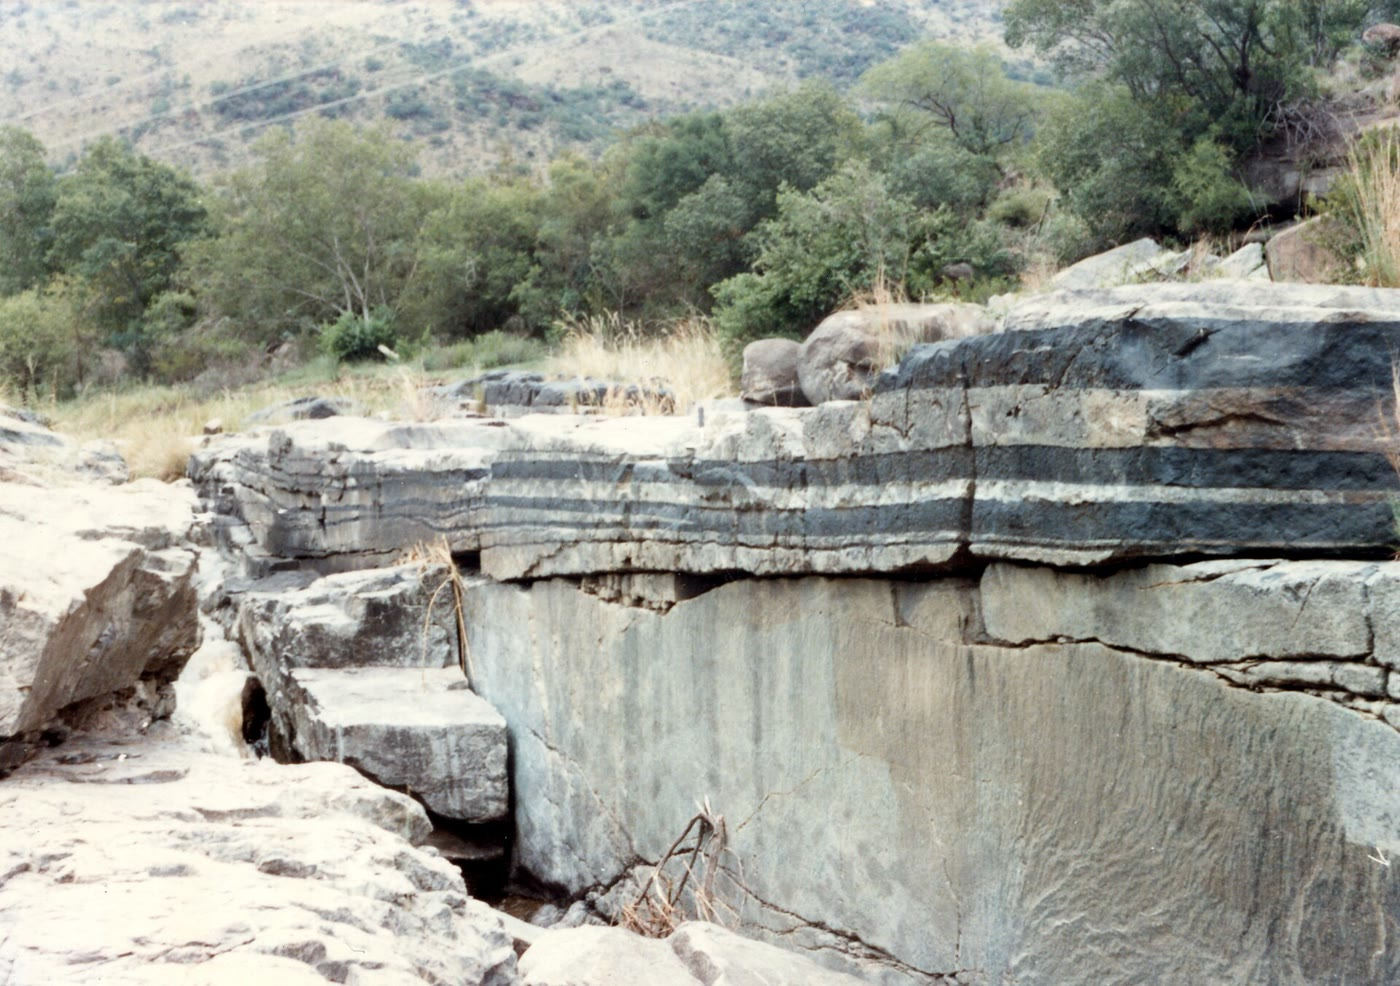
\includegraphics[height=5.2cm]{images/book4/b2-bushveld-chromitite.jpg}
\end{minipage}\hfill
\begin{minipage}[t]{0.42\linewidth}\vspace{0pt}\centering
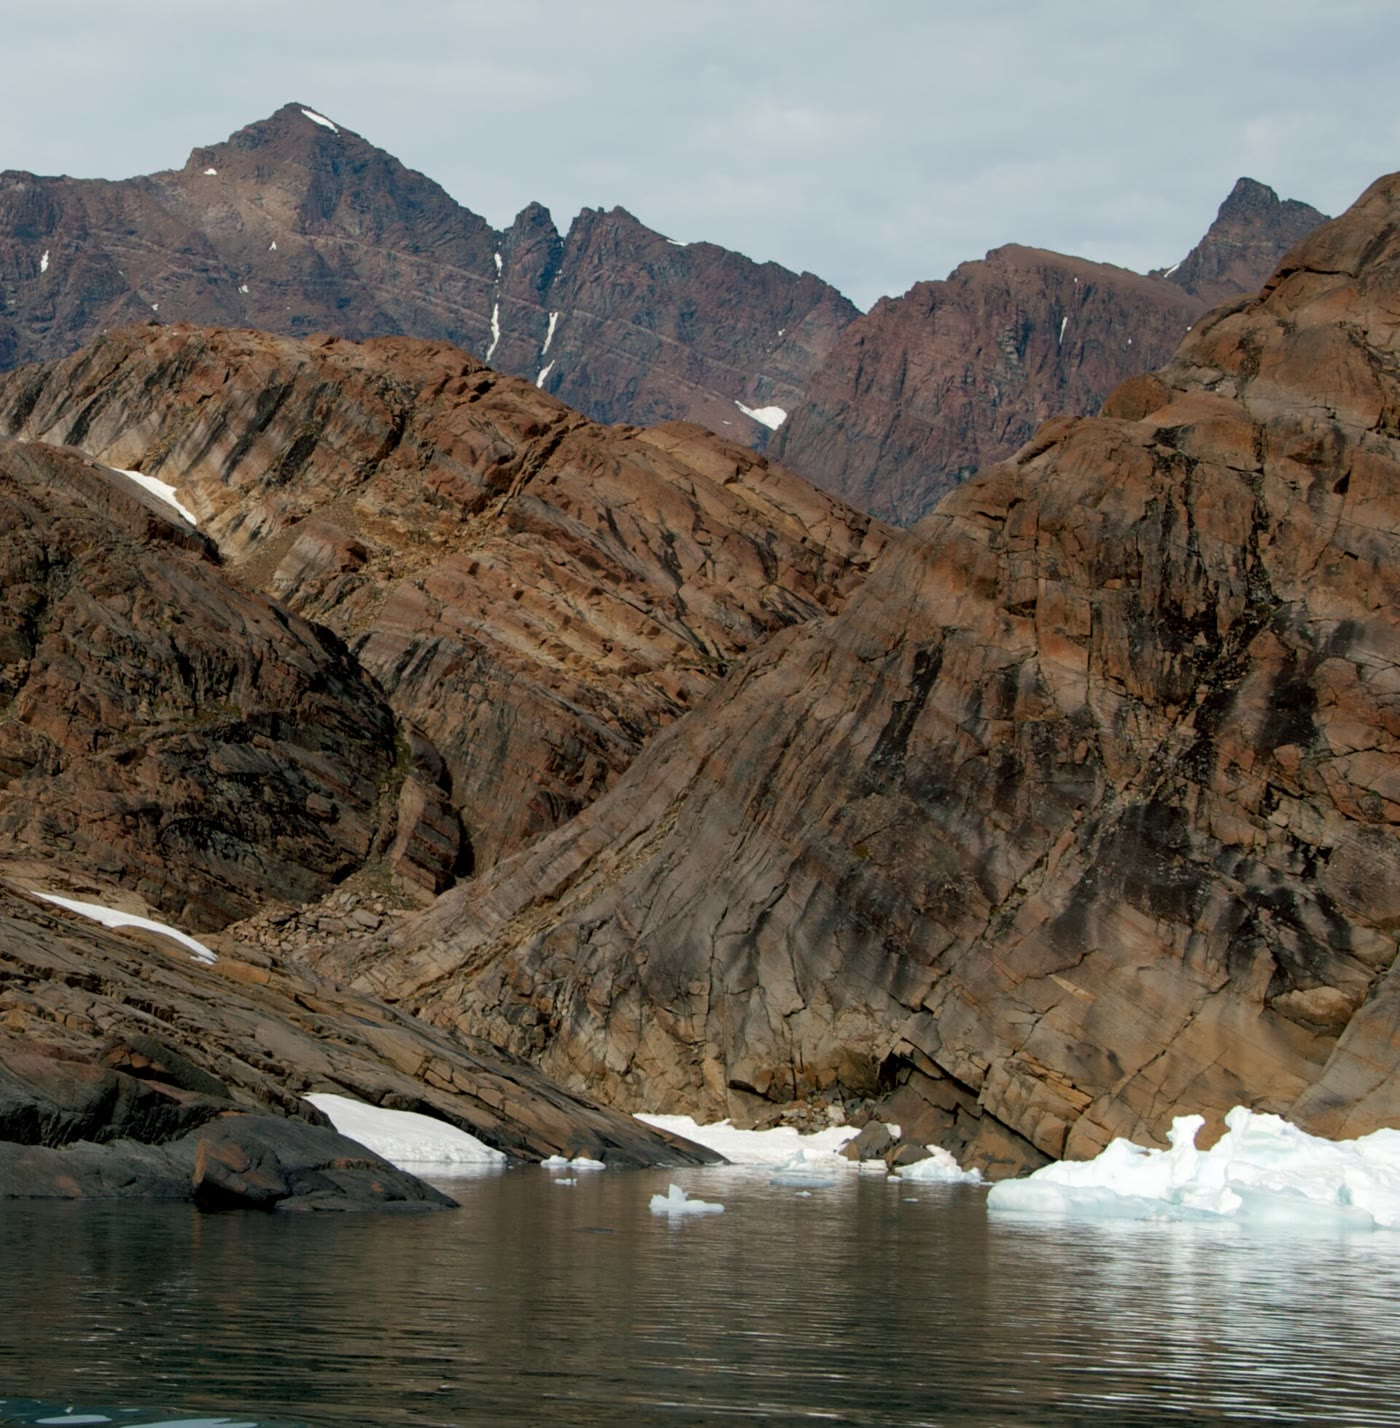
\includegraphics[height=5.2cm]{images/book4/b2-skaergaard-layering.jpg}
\end{minipage}
\par\smallskip{\small 左：南非布什维尔德杂岩临界带中的黑色铬铁岩层与灰色斜长岩层
（Kevin Walsh，CC BY 2.0）。右：东格陵兰斯卡尔加德侵入体中带的层状辉长岩，
自左上向右下倾斜
（C. Tegner，CC BY 4.0）。}
\end{omfigure}

\section{开口系统}\label{sec:b2:magmatic-differentiation:open}

\omterm{def:b2:magma-emplacement:magma}{岩浆}房很少是封闭的。新\omterm{def:b2:magma-emplacement:magma}{岩浆}从下方不断进入，
而\omterm{def:b2:magma-emplacement:magma}{岩浆}房的围岩是\omterm{def:b2:magma-emplacement:magma}{岩浆}能够加热、熔化并溶解的岩石。

\begin{definition}[岩浆混合；地壳同化；AFC]
\label{def:b2:magmatic-differentiation:open}
\emph{岩浆混合}\index{岩浆混合}是指两种成分不同的\omterm{def:b2:magma-emplacement:magma}{岩浆}
混合为一体。\emph{地壳同化}\index{地壳同化}是指地壳岩石
通过围岩或落入\omterm{def:b2:magma-emplacement:magma}{岩浆}中块体的熔化与溶解而并入\omterm{def:b2:magma-emplacement:magma}{岩浆}。
\emph{同化–分离结晶}\index{同化–分离结晶}（AFC）是二者
在同一\omterm{def:b2:magma-emplacement:magma}{岩浆}房中的组合：\omterm{def:b2:magma-emplacement:magma}{岩浆}结晶，
释放的潜热使
围岩熔化并被同化。
\end{definition}

\begin{proposition}[混合在浓度上是线性的]\label{prop:b2:magmatic-differentiation:mixing}
由质量分数为 $s$ 的\omterm{def:b2:magma-emplacement:magma}{岩浆} A 与质量分数为 $1-s$ 的\omterm{def:b2:magma-emplacement:magma}{岩浆} B 组成的混合物，其每一浓度
$C = sC_A + (1-s)C_B$：在一种浓度对另一种浓度的任一图解上，
混合物位于由 A 到 B 的直线段上，
且由杠杆规则可得 $s$。
\end{proposition}

\begin{proof}
每种元素都是守恒的：$C(m_A + m_B) = m_AC_A + m_BC_B$；两边除以 $m_A + m_B$。
\end{proof}

混合与晶体移除在\omterm{def:b2:magmatic-differentiation:harker}{哈克图解}上都画出直线，同位素比值
可以将二者区分开。结晶不改变同位素比值，而与比值不同的岩石混合则会改变，
其轨迹为双曲线（见
\cref{ch:b2:isotope-geochemistry}）。因此，在火山岩系列中，$^{87}$Sr/$^{86}$Sr 随
二氧化硅含量升高，即是\omterm{def:b2:magmatic-differentiation:open}{地壳同化}的标志。

\begin{proposition}[同化与分离结晶]
\label{prop:b2:magmatic-differentiation:afc}
\omterm{def:b2:magma-emplacement:magma}{岩浆}结晶出对某元素总分配系数为 $D$ 的晶体，并
同化浓度为 $C_a$ 的围岩，同化速率为结晶速率的 $r$ 倍
（$r \ne 1$）。设 $F$ 为\omterm{def:b2:magma-emplacement:magma}{岩浆}质量与其初始质量之比，
$z = (r + D - 1)/(r - 1)$，则
\[
\frac{C}{C_0} = F^{-z} + \frac{r}{r - 1 + D}\,\frac{C_a}{C_0}\,\bigl(1 - F^{-z}\bigr).
\]
当 $r = 0$ 时，此即\omterm{thm:b2:magmatic-differentiation:rayleigh}{瑞利分馏定律}。\omterm{def:b2:magma-emplacement:magma}{岩浆}中该元素的同位素比值
是初始\omterm{def:b2:magma-emplacement:magma}{岩浆}与围岩的同位素比值的平均，以
上式的两项为权重。
\end{proposition}

\begin{proof}
以初始质量为单位，当质量 $\mathrm dm_c$ 结晶时，同化的质量为
$r\,\mathrm dm_c$，\omterm{def:b2:magma-emplacement:magma}{岩浆}质量的变化为 $\mathrm dM =
-(1-r)\,\mathrm dm_c$。元素平衡为 $\mathrm d(MC) = rC_a\,\mathrm dm_c -
DC\,\mathrm dm_c$。展开左边，并将 $\mathrm dm_c$ 以
$-\mathrm dM/(1-r)$ 代入，得
\[
M\frac{\mathrm dC}{\mathrm dM} = -C - \frac{rC_a - DC}{1-r}
= \frac{(r - 1 + D)\,C - rC_a}{1 - r} = -z\,\bigl(C - C^*\bigr),
\qquad C^* = \frac{rC_a}{r - 1 + D}.
\]
于是 $\mathrm d(C - C^*)/(C - C^*) = -z\,\mathrm dM/M$，且 $C - C^*$ 与
$M^{-z}$ 成正比；由初值 $C = C_0$（$M = 1$），得 $C = C^* + (C_0 - C^*)F^{-z}$，
即上式。当 $r = 0$ 时，$z = 1 - D$，$C^* = 0$。来自初始\omterm{def:b2:magma-emplacement:magma}{岩浆}的原子
服从同一方程，令 $C_a = 0$，故其浓度为
$C_0F^{-z}$；其余原子来自围岩，这正是同位素比值按上述方式加权的原因。
\end{proof}

德保罗于 1981 年给出这些方程，它们是描述\omterm{def:b2:magma-emplacement:magma}{岩浆}
在穿越地壳途中受混染的标准模型。它们隐含着一个热约束。热量
用于同化岩石，来自晶体的潜热：将地壳岩石加热
从 150 升至 \qty{1150}{\celsius} 约需 \qty{1}{kJ/g}，熔化它需 \qty{300}{J/g}，
而\omterm{def:b2:magma-emplacement:magma}{岩浆}结晶释放约 \qty{400}{J/g}；因此每同化一克岩石，
约需 \qty{3.25}{g} \omterm{def:b2:magma-emplacement:magma}{岩浆}结晶，故 $r$ 远小于 1。
威尔科克斯对帕里库廷火山做过同样的计算：他的 \qty{25.4}{g} 石英二长岩，
温度约为 \qty{200}{\celsius}，需约 \qty{31350}{J} 才能
被加热至 \qty{1100}{\celsius} 并熔化，而结晶约
\qty{85}{g} 斜长石所释放的热量远超其质量平衡所移除的
\qty{12.5}{g} 晶体。喷出的\omterm{def:b2:magma-emplacement:magma}{岩浆}不可能自行支付同化所需的热量：
热量必定来自一个比喷出\omterm{def:b2:magma-emplacement:magma}{岩浆}更大的\omterm{def:b2:magma-emplacement:magma}{岩浆}体，
它在视线之外结晶（见\cref{exo:b2:magmatic-differentiation:11}）。
% ledger: depaolo81:afc, white09:afc-heat, wilcox54:heat, wilcox54:mass-balance

\begin{omfigure}
\centering
\begin{tikzpicture}
\begin{axis}[omrecord, name=left, width=0.47\linewidth, height=5.4cm,
  xmin=0.3, xmax=1, ymin=0.3, ymax=1.05, x dir=reverse,
  xlabel={剩余岩浆 $F$}, ylabel={Sr: $C/C_0$},
  tick label style={font=\scriptsize}, label style={font=\small}]
\addplot[thick, black] table[x=F, y=srC_r0] {figdata/out/bachelor-2-differentiation-afc.dat};
\addplot[thick, blue!70!black] table[x=F, y=srC_r02] {figdata/out/bachelor-2-differentiation-afc.dat};
\addplot[thick, red!70!black] table[x=F, y=srC_r05] {figdata/out/bachelor-2-differentiation-afc.dat};
\end{axis}
\begin{axis}[omrecord, at={(left.east)}, anchor=west, xshift=1.7cm,
  width=0.47\linewidth, height=5.4cm,
  xmin=0.3, xmax=1, ymin=0.703, ymax=0.716, x dir=reverse,
  xlabel={剩余岩浆 $F$}, ylabel={$^{87}$Sr/$^{86}$Sr},
  y tick label style={/pgf/number format/fixed, /pgf/number format/precision=3},
  legend style={font=\scriptsize, at={(0.03,0.97)}, anchor=north west},
  tick label style={font=\scriptsize}, label style={font=\small}]
\addplot[thick, black] table[x=F, y=iso_r0] {figdata/out/bachelor-2-differentiation-afc.dat};
\addlegendentry{$r = 0$}
\addplot[thick, blue!70!black] table[x=F, y=iso_r02] {figdata/out/bachelor-2-differentiation-afc.dat};
\addlegendentry{$r = 0.2$}
\addplot[thick, red!70!black] table[x=F, y=iso_r05] {figdata/out/bachelor-2-differentiation-afc.dat};
\addlegendentry{$r = 0.5$}
\end{axis}
\end{tikzpicture}
\par\smallskip{\small 同化与\omterm{def:b2:magmatic-differentiation:crystallisation}{分离结晶}，以锶为例
（$D = 1.5$，围岩的锶含量为\omterm{def:b2:magma-emplacement:magma}{岩浆}的一半，
$^{87}$Sr/$^{86}$Sr = 0.7200，\omterm{def:b2:magma-emplacement:magma}{岩浆}为 0.7035；示意性数值）。左：
浓度随同化速率 $r$ 增大而下降得更快，因为围岩带入的锶更少，
同一 $F$ 下形成的晶体更多。右：同位素比值，
仅靠结晶时不变（$r = 0$），向围岩的比值攀升。}
\end{omfigure}

\section{读取环带晶体}\label{sec:b2:magmatic-differentiation:zoning}

\begin{definition}[成分环带]\label{def:b2:magmatic-differentiation:zoning}
固溶体晶体的成分若从核心到边缘发生变化，即称其具有\emph{成分环带}\index{成分环带}，
它记录了各层生长时所依据的液相的变化。
当边缘富含低温组分（斜长石中的钠）时，称为\emph{正环带}；
边缘富含高温组分时，称为\emph{反环带}；
成分交替出现时，称为\emph{振荡环带}。
\end{definition}

环带晶体即正在进行的\omterm{def:b2:magmatic-differentiation:crystallisation}{分离结晶}的现场记录：其核心未能
与后期液相重新达到平衡。下图在鲍文反应环上计算了
由含 \qty{50}{\percent} 钙长石的液相生长出的斜长石。\omterm{def:b2:magmatic-differentiation:crystallisation}{平衡结晶}时，
晶体始终均匀，最终成分为 \qty{50}{\percent}；完全\omterm{def:b2:magmatic-differentiation:crystallisation}{分离结晶}时，
每一新生层都与越来越富钠的液相处于平衡，
最后形成的晶体边缘几乎是纯钠长石。正环带，自钙质核心到钠质边缘，
正是鲍文系列对冷却\omterm{def:b2:magma-emplacement:magma}{岩浆}的预测。反环带，即
在钠质环带外侧出现的钙质环带，说明晶体突然被更热或更富钙的液体包围：
这往往意味着新\omterm{def:b2:magma-emplacement:magma}{岩浆}注入，
在\omterm{def:b2:magma-emplacement:magma}{岩浆}房中与原有\omterm{def:b2:magmatic-differentiation:open}{岩浆混合}的结果。
% ledger: bowen13:plagioclase, earle:bowen (Book 2)

\begin{omfigure}
\centering
\begin{tikzpicture}
\begin{axis}[omrecord, width=0.78\linewidth, height=6cm,
  xmin=0, xmax=1, ymin=0, ymax=90,
  xlabel={已结晶液相的比例},
  ylabel={钙长石（\unit{\percent}，分子）},
  legend style={font=\scriptsize, at={(0.02,0.02)}, anchor=south west},
  tick label style={font=\scriptsize}, label style={font=\small}]
\addplot[very thick, red!70!black] table[x=x, y=an_frac] {figdata/out/bachelor-2-differentiation-zoning.dat};
\addlegendentry{分离结晶：新生层}
\addplot[thick, gray, densely dotted] table[x=x, y=an_liq_frac] {figdata/out/bachelor-2-differentiation-zoning.dat};
\addlegendentry{分离结晶：液相}
\addplot[very thick, blue!70!black, dashed] table[x=x, y=an_eq] {figdata/out/bachelor-2-differentiation-zoning.dat};
\addlegendentry{平衡结晶：晶体}
\end{axis}
\end{tikzpicture}
\par\smallskip{\small 由含 \qty{50}{\percent}
钙长石的液相结晶出的斜长石，据鲍文（1913）的反应环计算。\omterm{def:b2:magmatic-differentiation:crystallisation}{分离结晶}中，
晶体各层自核心（左）到边缘（右）越来越富钠，
当约 \qty{82}{\percent} 已结晶时，液相达到钠长石成分；
\omterm{def:b2:magmatic-differentiation:crystallisation}{平衡结晶}中，晶体保持均匀，
最终成分与其来源液相的成分相同。}
\end{omfigure}

\begin{inthelab}[读取环带晶体]
岩石学家先在正交偏光下观察环带，此时斜长石的各环带
以略有不同的角度消光，并呈现为同心条带。
随后进行测量：电子探针（见\cref{ch:b2:field-lab-methods-2}）
沿自核心至边缘的剖面，分析直径仅几微米的微区，并作
钙与钠的分布图可直接显示各环带。由此剖面，
可借助上图的反应环或分配系数，计算各环带生长时所来自的液相成分，
并将反环带的数目计为\omterm{def:b2:magma-emplacement:magma}{岩浆}房的
补给次数。沿同一剖面用激光剥蚀测得的\omterm{def:b2:elements-in-the-earth:trace}{微量元素}，
与逐环带测得的同位素比值一起，可区分单个晶体历史中的
\omterm{def:b2:magmatic-differentiation:crystallisation}{分离结晶}、混合与同化作用。
\end{inthelab}

\section{练习}

\begin{exercise}[$\star$]\label{exo:b2:magmatic-differentiation:1}
利用鲍文对斜长石的测量数据（固相线 / 液相线，\unit{\celsius}）：
An$_{100}$ 1550 / 1550；An$_{83.3}$ 1465 / 1521；An$_{66.7}$ 1372 / 1490；An$_{50}$
1287 / 1450；An$_{33.3}$ 1205 / 1394；An$_{20}$ 液相线 1334；An$_{11.1}$ 液相线
1265，在相邻数据点之间作线性插值。考虑一含
\qty{50}{\percent} 钙长石的液相，在平衡条件下冷却。（a）该液相于何温度
开始结晶，首个晶体的成分是什么？（b）
在 \qty{1394}{\celsius} 时，液相与晶体的成分各是什么，
以及已结晶的质量分数是多少（将摩尔分数当作质量分数使用）？
（c）最后一滴液相的成分是什么？
\end{exercise}
% ledger: bowen13:plagioclase

\begin{exercise}[$\star$]\label{exo:b2:magmatic-differentiation:2}
一个辉长质\omterm{def:b2:magmatic-differentiation:cumulate}{堆晶岩}含 \qty{50}{\percent} 斜长石、\qty{35}{\percent}
单斜辉石和 \qty{15}{\percent} 橄榄石。分配系数为
（橄榄石 / 单斜辉石 / 斜长石）Sr 0.000063 / 0.157 / 2.7，Zr 0.00068 /
0.195 / 0.001 和 Rb 0.000044 / 0.0033 / 0.025，计算各元素的总分配
系数，并指出哪一种元素是\omterm{def:b2:elements-in-the-earth:partition}{相容元素}。
\end{exercise}
% ledger: white07:kd-basalt

\begin{exercise}[$\star$]\label{exo:b2:magmatic-differentiation:3}
\omterm{def:b2:magmatic-differentiation:cumulate}{堆晶岩}（见\cref{exo:b2:magmatic-differentiation:2}）由玄武岩经\omterm{def:b2:magmatic-differentiation:crystallisation}{分离结晶}形成，
直至剩下一半液相。（a）Sr、Zr 与 Rb 在液相中各改变了多少倍
（取总分配系数分别为 1.40、0.069 和 0.014）？（b）
Zr/Rb 比值改变了多少倍？请结合关于比值的推论加以说明。
\end{exercise}
% ledger: white07:kd-basalt

\begin{exercise}[$\star$]\label{exo:b2:magmatic-differentiation:4}
Parícutin 火山 1943 年 2 月的首批熔岩含 \qty{55.04}{\percent} \ce{SiO2}，
\qty{5.68}{\percent} \ce{MgO} 和 \qty{0.85}{\percent} \ce{K2O}；末批（
1952 年 2 月）的值分别为 60.07、3.73 和 \qty{1.67}{\percent}。（a）求各氧化物的变化量。
（b）氧化钾不进入任何结晶矿物。若其浓集仅由\omterm{def:b2:magmatic-differentiation:crystallisation}{分离结晶}造成，
则液相中剩余的比例应为多少？
（c）威尔科克斯的质量平衡仅需移除约 \qty{12.5}{g} 晶体，
即每 \qty{100}{g} \omterm{def:b2:magma-emplacement:magma}{岩浆}。该比较说明了什么？
\end{exercise}
% ledger: wilcox54:table2, wilcox54:mass-balance

\begin{exercise}[$\star\star$]\label{exo:b2:magmatic-differentiation:5}
比较\omterm{def:b2:magmatic-differentiation:crystallisation}{分离结晶}与\omterm{def:b2:magmatic-differentiation:crystallisation}{平衡结晶}：分别依两种定律计算 $C_L/C_0$
（a）对镍，$D = 5$，当液相的 \qty{20}{\percent} 已结晶时；（b）
对\omterm{def:b2:elements-in-the-earth:partition}{不相容元素}，$D = 0.01$，当 \qty{90}{\percent} 已结晶时。
（c）当 $F \to 0$ 时，两种定律的极限各是什么？哪一种定律能
把液相中的\omterm{def:b2:elements-in-the-earth:partition}{相容元素}完全除去？
\end{exercise}

\begin{exercise}[$\star\star$]\label{exo:b2:magmatic-differentiation:6}
（a）计算橄榄石中 \ce{MgO}、\ce{FeO} 和 \ce{SiO2} 的质量百分数，
Fo$_{80}$，$(\ce{Mg}_{0.8}\ce{Fe}_{0.2})_2\ce{SiO4}$（$M$ = 40.30、71.84 和
\qty{60.08}{g/mol}）。（b）某玄武岩含 \qty{10.0}{\percent} \ce{MgO} 和
\qty{49.0}{\percent} \ce{SiO2}，仅结晶出此橄榄石，直至其液相
\qty{8.0}{\percent} \ce{MgO}。被移出的橄榄石质量分数为多少？（c）
求此时液相的二氧化硅含量？
\end{exercise}

\begin{exercise}[$\star\star$]\label{exo:b2:magmatic-differentiation:7}
对斯凯尔加德侵入体，$F = \num{1.091e-7}H^2 - \num{5.9064e-4}H + 0.7678$。
（a）求 $F$ 在 $H = 0$、1000 和 \qty{2000}{m} 处的值。（b）$F = 0$ 时的高度为多少？
（c）出露的底板层序底部形成之前，已结晶的\omterm{def:b2:magma-emplacement:magma}{岩浆}占多大比例，
它可能位于何处？
\end{exercise}
% ledger: tegner23:skaergaard

\begin{exercise}[$\star\star$]\label{exo:b2:magmatic-differentiation:8}
沿斯凯尔加德剖面，中位\omterm{def:b2:magmatic-differentiation:cumulate}{堆晶岩}的镍含量为：
$F = 0.70$ 时（下部带 a）\qty{177}{ppm}，$F = 0.29$ 时（中部带）\qty{54}{ppm}，以及
$F = 0.17$ 时（上部带 a）\qty{6.2}{ppm}。（a）假设\omterm{def:b2:magmatic-differentiation:cumulate}{堆晶岩}所含镍为其液相的
$D$ 倍，且液相服从瑞利定律，
求前两层之间的表观 $D$。（b）对后两层作同样的
计算。（c）什么因素会使表观 $D$ 发生变化？
\end{exercise}
% ledger: data:b4-skaergaard

\begin{exercise}[$\star\star$]\label{exo:b2:magmatic-differentiation:9}
核对威尔科克斯的答案：第一期熔岩的 \qty{100}{g} 基质（\ce{SiO2}
55.53，\ce{MgO} 4.66，\ce{K2O} \qty{0.88}{\percent}），加上 \qty{25.4}{g} 平均
捕虏体（72.48、0.77、3.64），减去 \qty{2.9}{g} 橄榄石 Fo$_{80}$（39.19、42.06、0）
再减去 \qty{9.6}{g} 斜长石 An$_{70}$（50.54、0、0）。（a）剩余质量为多少？
（b）计算其 \ce{SiO2}、\ce{MgO} 和 \ce{K2O}，并与
熔岩 19 的基质（60.16、3.19 和 \qty{1.75}{\percent}）比较。（c）哪一种氧化物符合得最差？
\end{exercise}
% ledger: wilcox54:groundmass, wilcox54:xenoliths, wilcox54:mass-balance

\begin{exercise}[$\star\star\star$]\label{exo:b2:magmatic-differentiation:10}
一\omterm{def:b2:magma-emplacement:magma}{岩浆}在结晶的同时同化围岩，取 $r = 0.2$，$D_{\ce{Sr}} =
1.5$，$C_a/C_0 = 0.5$，初始 $^{87}$Sr/$^{86}$Sr = 0.7035，围岩为 0.7200。
（a）计算 $z$、$F^{-z}$ 及 $C/C_0$（$F = 0.7$）。（b）与同一 $F$ 下的纯\omterm{def:b2:magmatic-differentiation:crystallisation}{分离
结晶}相比，并结合两种情况下所形成晶体的质量解释其差异。
（c）计算\omterm{def:b2:magma-emplacement:magma}{岩浆}的 $^{87}$Sr/$^{86}$Sr。
\end{exercise}

\begin{exercise}[$\star\star\star$]\label{exo:b2:magmatic-differentiation:11}
依威尔科克斯对帕里库廷火山的热量收支：（a）一克石英
二长岩由 200 升温至 \qty{1100}{\celsius} 所需热量（热容
\qty{1.1}{J/(g.K)}），再熔化（\qty{250}{J/g}）所需热量？（b）
\qty{25.4}{g} 需多少热量？（c）若斜长石 An$_{70}$（潜热 \qty{370}{J/g}）
须结晶出多少质量？（d）与质量平衡中的 \qty{12.5}{g} 晶体量比较，
计算同化量与结晶量之比 $r$，
并说明这意味着什么。
\end{exercise}
% ledger: wilcox54:heat, white09:afc-heat

\begin{exercise}[$\star\star\star$]\label{exo:b2:magmatic-differentiation:12}
某玄武岩含镍 \qty{250}{ppm}，先仅结晶橄榄石（$D = 5$），直至
$F = 0.8$，随后结晶橄榄石、斜长石和单斜辉石（总 $D = 1.5$）。（a）
计算镍在各阶段的变化倍数，以及
$F = 0.5$ 时液相的镍含量。（b）若只用 $D = 5$ 的单一定律，会得出怎样的预测？
（c）说明为何瑞利定律须分阶段应用。
\end{exercise}

\section{问题：写下自身历史的侵入体}

\begin{problem}[{周末问题——由辉长岩的层序推算最终
仍为液态的岩浆所占比例}]
\label{pb:b2:magmatic-differentiation:1}
一（虚构的）层状辉长岩\omterm{def:b2:magma-emplacement:bodies}{岩床}，由一玄武岩结晶而成，该玄武岩的\omterm{def:b2:magma-emplacement:aureole}{冷凝边}
给出母岩成分：\ce{SiO2} 49.5，\ce{Al2O3} 16.0，\ce{FeO} 10.0，
\ce{MgO} 9.0，\ce{CaO} 11.5，\ce{Na2O} 2.5，\ce{K2O} \qty{0.30}{\percent}；
\qty{150}{ppm} 镍和 \qty{80}{ppm} 锆。下部带\omterm{def:b2:magmatic-differentiation:cumulate}{堆晶岩}由
\qty{20}{\percent} 橄榄石、\qty{50}{\percent} 斜长石和 \qty{30}{\percent}
单斜辉石组成；橄榄石消失层位以上则由 \qty{55}{\percent}
斜长石和 \qty{45}{\percent} 单斜辉石组成。取分配系数
（橄榄石 / 斜长石 / 单斜辉石）镍 5.0 / 0 / 2.0，锆 0.0007 / 0.001 /
0.195。矿物成分（\unit{\percent}）：橄榄石 \ce{MgO} 42.06，\ce{CaO} 0，
\ce{Al2O3} 0，\ce{SiO2} 39.19；斜长石 0、14.36、31.70、50.54；单斜辉石
16.0、20.5、3.0、51.5。一条\omterm{def:b2:magma-emplacement:bodies}{岩墙}
由细粒岩石构成的\omterm{def:b2:magma-emplacement:bodies}{岩墙}，在最上层结晶时由\omterm{def:b2:magma-emplacement:magma}{岩浆}房补给，其
成分为 \ce{SiO2} 50.0，\ce{Al2O3} 14.1，\ce{FeO} 16.7，\ce{MgO} 4.9，\ce{CaO} 7.3，
\ce{Na2O} 3.4，\ce{K2O} \qty{0.75}{\percent} 及 \qty{188}{ppm} 锆。

\noindent\textbf{第一部分——各层的分配系数。}
\begin{enumerate}
\item 计算下部带中镍的总分配系数。
\item 计算下部带中锆的总分配系数。
\item 计算上部带中二者的总分配系数。
\item 各带中哪种元素为\omterm{def:b2:elements-in-the-earth:partition}{相容元素}？镍在
橄榄石消失后是否仍为\omterm{def:b2:elements-in-the-earth:partition}{相容元素}？
\item \omterm{def:b2:magmatic-differentiation:cumulate}{堆晶岩}中的锆主要集中于哪种矿物？为什么？
\item 下部带中，$F$ 每减半一次，液相中 Ni/Zr 比值
改变的倍数是多少？
\end{enumerate}

\noindent\textbf{第二部分——沿剖面向上的瑞利曲线。}
\begin{enumerate}[resume]
\item 在 $F = 1$ 时结晶形成的最底部\omterm{def:b2:magmatic-differentiation:cumulate}{堆晶岩}中，
预期镍含量为多少？
\item 位置较高的下部带\omterm{def:b2:magmatic-differentiation:cumulate}{堆晶岩}含镍 \qty{190}{ppm}，它形成于
$F$ 为何值时？
\item 此时液相中的锆含量为多少？
\item 在该 $F$ 下，比较由\omterm{def:b2:magmatic-differentiation:crystallisation}{分离结晶}定律与
\omterm{def:b2:magmatic-differentiation:crystallisation}{平衡结晶}定律分别给出的液相镍含量。
\item 橄榄石在 $F = 0.55$ 时消失，计算该处
液相的镍含量。
\item 计算该层位正下方和正上方形成的\omterm{def:b2:magmatic-differentiation:cumulate}{堆晶岩}
镍含量。地质学家在剖面中会看到怎样的特征？
\item 计算 $F = 0.40$ 时液相与\omterm{def:b2:magmatic-differentiation:cumulate}{堆晶岩}的镍含量，
并解释其变化趋势。
\end{enumerate}

\noindent\textbf{第三部分——最后残余液体的质量平衡。}
\begin{enumerate}[resume]
\item 对一种氧化物写出方法的守恒方程，设
$x_{\mathrm{ol}}, x_{\mathrm{pl}}, x_{\mathrm{cpx}}$ 为每 \qty{100}{g} 母岩中被移除的
矿物质量，并以\omterm{def:b2:magma-emplacement:bodies}{岩墙}为子体。
\item 分别对 \ce{MgO}、\ce{CaO} 和 \ce{Al2O3} 写出该方程。
\item 解 $3 \times 3$ 方程组。
\item 母岩中有多大比例以液体形式残留？
\item 用 \ce{SiO2} 检验结果：由所求质量重新计算液相的
二氧化硅含量。
\item 将所移除矿物的比例与两个带的
矿物模式作比较。
\item 钾不进入任何一种矿物：由此得到的液相比例为多少？
\end{enumerate}

\noindent\textbf{第四部分——顶部的液相比例。}
\begin{enumerate}[resume]
\item 橄榄石于
$F = 0.55$ 时消失，液相中的锆升高了多少倍？此时锆含量为多少？
\item 由\omterm{def:b2:magma-emplacement:bodies}{岩墙}的锆含量，计算其形成时残留的液体比例，
并应用自 $F = 0.55$ 起的上部带定律。
\item 从头取单一的 $D = 0.07$ 重做计算，结果
是否对 $D$ 的具体取值敏感？
\item 液相中的铁由 10.0 升至 \qty{16.7}{\percent}，而
二氧化硅几乎不变。哪些矿物应对此负责？这预示着哪一类\omterm{def:b2:magma-emplacement:magma}{岩浆}系列
（见\cref{ch:b2:magmatic-series}）？
\item 最上部\omterm{def:b2:magmatic-differentiation:cumulate}{堆晶岩}含 \qty{47}{ppm} 的 Zr。若仅由堆晶晶体构成，其含锆量应为液相的
$\bar D$ 倍。捕虏液体的质量分数为多少，
（成分与\omterm{def:b2:magma-emplacement:bodies}{岩墙}相同）才能解释该分析结果？
\item 给出最上层结晶时仍为液体的原始\omterm{def:b2:magma-emplacement:magma}{岩浆}比例，
即本题的关键数值，并比较三种估计：
（主量元素、钾、锆）。
\end{enumerate}
\end{problem}
% ledger: white07:kd-basalt, matzen12:dni
